\documentclass[landscape]{article}

\usepackage{tboxen}
\usepackage{amsmath}
\usepackage{amssymb}
\usepackage{epsfig}
\usepackage[tight]{subfigure}
\usepackage{color}
\usepackage{type1cm}
\usepackage{tabularx}
\usepackage{subfig}

% Custom variables

% How much length we want to add to the poster while editing.  Note
% that these are just integer variables.  There is probably a better
% way to do this...
\newcounter{width}
\newcounter{height}
\newcounter{extra-length}
% these are in cm
\setcounter{width}{110}
\setcounter{height}{68} % developing at 2/3 magnification for 40x65in poster
\setcounter{extra-length}{0} % for development

% Boolean variable: whether or not we want to show grid lines
\newif\ifusegrid
\usegridtrue
\usegridfalse

% You can define any rgb colors you want for the background.  The
% first two lines define a blue to cream fade.  See how they are used
% below.
\definecolor{bottomcolor}{rgb}{ 0.538, 0.663, .788}
\definecolor{topcolor}{rgb}{    0.538, 0.663, .788}
% Uncomment these next two lines if you want to have an all white background.
% TODO: temp dev setting
%\definecolor{topcolor}{rgb}{1,1,1}
%\definecolor{bottomcolor}{rgb}{1,1,1}

% Other counters that we will use below.
\newcounter{grid-top}
\newcounter{grid-right}
\newcounter{title-top}
\newcounter{title-left-margin}
\newcounter{title-width}
\newcounter{title-left}
\newcounter{title-box-width}

% ==============================================================================
% Set up paper sizes

\newcounter{total-height}
\setcounter{total-height}{\arabic{height} + \arabic{extra-length}}
\setlength{\paperwidth}{\arabic{width}cm}
\setlength{\paperheight}{\arabic{total-height}cm}
\setlength{\textwidth}{\paperwidth}
\setlength{\textheight}{\paperheight}

% These usually stay the same for tboxen
\setlength{\headheight}{0 cm}
\setlength{\headsep}{0 cm}
\setlength{\topmargin}{-2 cm} 
\setlength{\oddsidemargin}{-1in}

% From tboxen:
% this is often necessary for pdf and dvips to work
\ifx\pdfoutput\undefined 
% for dvi
\special{papersize=\arabic{width}cm,\arabic{height}cm}
\else 
% for pdf
\pdfpagewidth=\paperwidth 
\pdfpageheight=\paperheight 
\fi 

% ==============================================================================
% POSTER STARTS HERE
\begin{document}
\begin{center}
  
  % ==============================================================================
  % Main body
  \begin{tikzpicture}
    
    % This defines your background box - entries are pretty self explanatory.
    % The colors ``topcolor'' and ``bottomcolor'' are defined above.
    \shade[top color = topcolor,
      bottom color = bottomcolor,
      rounded corners = 1cm, % The larger this is, the rounder your corners
      line width = 2mm, % The width of your border lines
      draw]
    (0,0) rectangle +(\textwidth-2cm,\textheight-1cm); 
    % This last line above just sets up the bounding box for the whole poster.  You don't want to change it.

    % ==============================================================================
    \ifusegrid
    % Draw grid guidelines if desired.
    \setcounter{grid-top}{\arabic{total-height}-1}
    \setcounter{grid-right}{\arabic{width}-2}
    \draw[style=help lines] (0,\arabic{extra-length}) grid (\arabic{grid-right},\arabic{grid-top});
    \setcounter{grid-top}{\arabic{height}-1}
    \foreach \x in {0,5,...,\arabic{grid-right}}
    \foreach \y in {0,5,...,\arabic{grid-top}}
    \draw (\x,\y) + (0,\arabic{extra-length}) node{\tiny \x,\y};
    \fi

    % ==============================================================================
    % Title box
    %
    % The following defaults make the title box span the whole top,
    % start 3cm from the top, and end 2 cm from both sides. I have
    % hard-coded the 2s and 3 below.  Play around with the trade-off
    % between changing these numbers and changing
    % ``title-left-margin'' if you are not happy with the defaults.
    \setcounter{title-left-margin}{0} % This specifies the additional padding to the right and left of the title.  Can be negative.
    \setcounter{title-top}{\arabic{total-height}-3} % Places the top of the title 3 cm from the top of the poster.
    \setcounter{title-width}{\arabic{width}-2*\arabic{title-left-margin} - 2*2 - 4} % Automatically calculates the width of the title based on the margin.
    \setcounter{title-left}{\arabic{title-left-margin} + 2} % Automatically places the title 2m from the left edge of the poster + the user specified margin.
    \setcounter{title-box-width}{\arabic{width} - 30}
    \path (\arabic{title-left},\arabic{title-top}) node(title) [style=tbox, text width=\arabic{title-width}cm] {
      \begin{center}

        % Three parboxes allow for images on both sides of the title
        % box with the title text in the middle.
        \parbox{10cm} {
        
\includegraphics[width=10cm]{../../figures/berkeley_seal.pdf}
        }
        \parbox{\arabic{title-box-width}cm} {
          \centering
              {\Huge \bf{Timely Object Recognition} } \\
              \vspace{1cm}
              \begin{tabular}{cccc}
                {\huge Sergey Karayev$^1$, \hfill} & {\huge Tobias Baumgartner$^2$, \hfill} & {\huge Mario Fritz$^3$, \hfill} & {\huge Trevor Darrell$^1$}\\
                \multicolumn{4}{c}{\Large $^1$UC Berkeley, $^3$RWTH Aachen, $^3$MPI Informatics}
              \end{tabular}
        }
        \parbox{10cm} {
          % This is just an empty box to make the actual title centered.
          % Add another seal or image if you wish.
          \hspace{1cm}
        }

      \end{center}
    };
    
    % ==============================================================================
    % ABSTRACT
    \path (title.south west) ++(0cm,-2cm) + (-\arabic{title-left-margin}cm,0cm) node(introduction) [style=tbox,text width=30cm] {
    \begin{itemize}
      \item Our task is multi-class object detection in a setting where there is not enough time to evaluate all detectors.

      \item We use reinforcement learning to learn a \emph{dynamic} policy for selecting detectors and classifiers.

      \item We evaluate detection performance vs. time with the novel \emph{timeliness} measure, and test on the PASCAL VOC challenge.
    \end{itemize}

    }; \addcenteredtitle{introduction}{Abstract} 
    % The above line adds the title ``Introduction'' to the box named ``introduction''.
    
    % ==============================================================================
    % FIGURE 1 WITH EXPLANATION 
    \path (introduction.south west) ++(0cm,-2cm) node(coding) [style=tbox,text width=30cm] {
      \begin{center}
        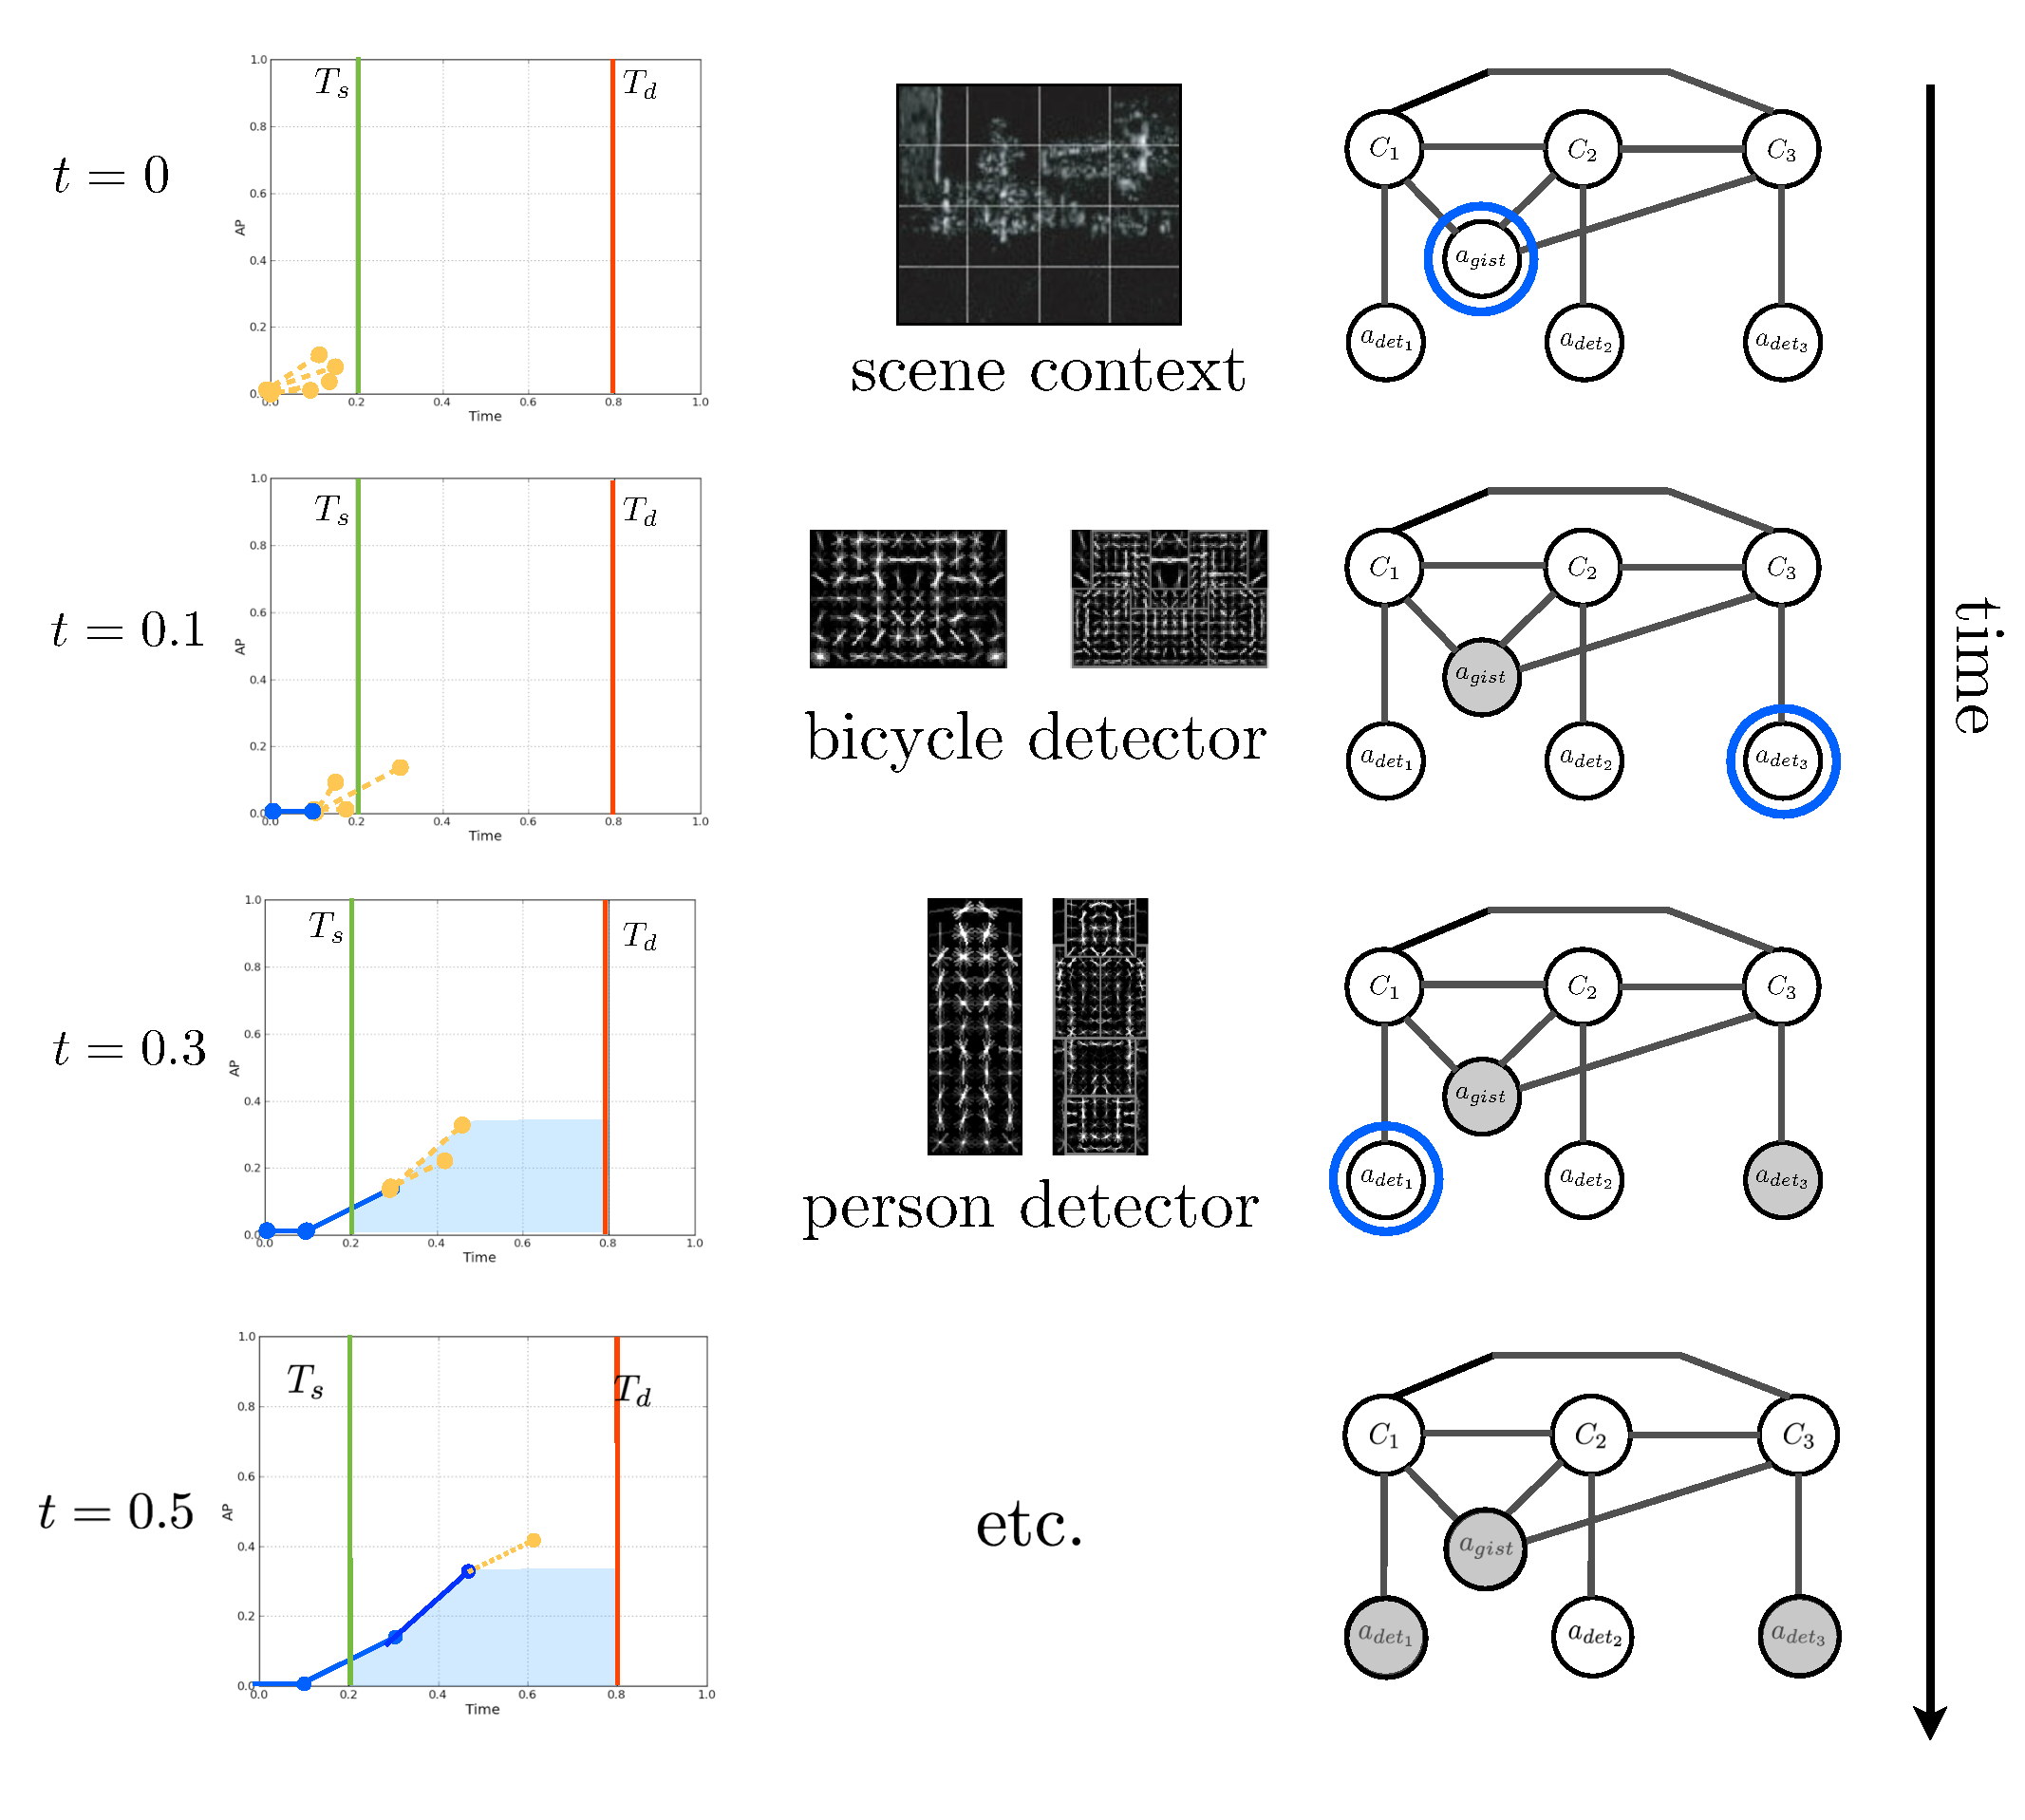
\includegraphics[width=26cm]{../../figures/figure1_extended.pdf}
      \end{center}

      \begin{itemize}
        \item Potential actions $a \in \mathcal{A}$ are considered according to their predicted \emph{value}.
        \item The value $Q(s,a)$ depends on the \emph{belief state} of the system as well as the action considered.
        \item The selected action returns observations (list of detections, or evaluated feature).
        \item Observations update the belief state through an inference process.
        \item The final evaluation is the area of the AP vs. Time curve between the start time $T_s$ and end time $T_d$.
        \item VOCalues are learned with reinforcement learning, using a reward function derived from this evaluation.
      \end{itemize}

    }; \addcenteredtitle{coding}{Sequential Detection}

    % ==============================================================================
    % Learning the Policy
    \path (introduction.north east) ++(2cm,0cm) node(model) [style=tbox,text width=34 cm] {
      % \begin{center}
      %   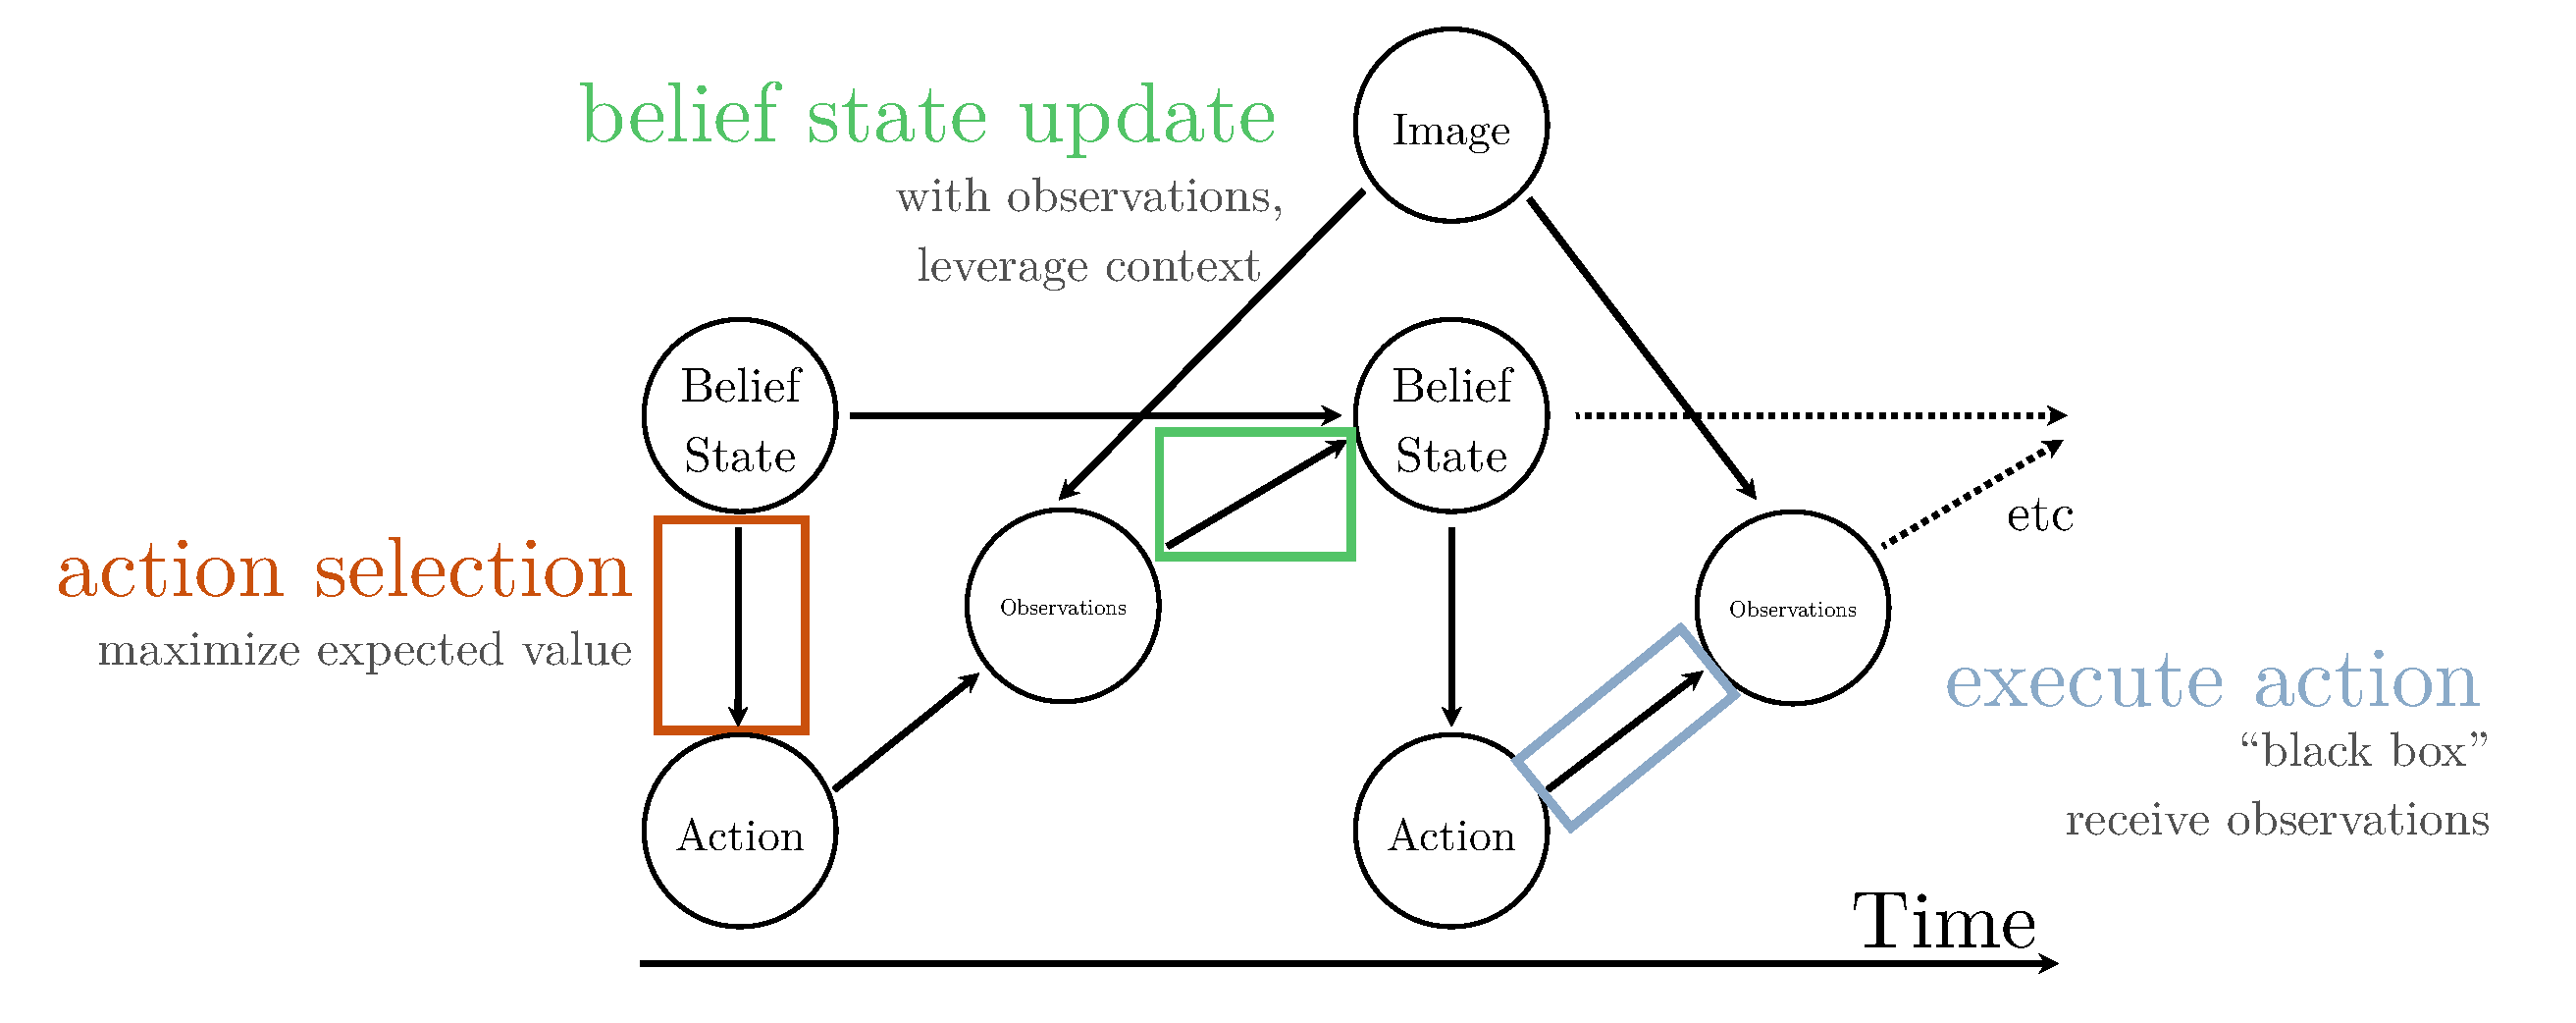
\includegraphics[width=20cm]{../../figures/pomdp_annotated.pdf}
      % \end{center}
      We define our policy as taking an untaken action with maximum value.
      \begin{align*} \pi(s) = \arg\max_{a_i \in \mathcal{A} \setminus \mathcal{O}} Q(s,a_i) = \theta_\pi^\top \phi(s,a) \end{align*}
      The Q-function is linearly approximated.
      \\

      \begin{center}\textbf{Reward Function}\end{center}

      \parbox{20cm}{
      The final performance evaluation of area under the AP vs. Time curve between $T_s$ and $T_d$ is additive per action.
      We define the reward function as
      \begin{align*} R(s^j,a) = \Delta \text{ap} (t_T^j-\frac{1}{2}\Delta t) \end{align*}}
      \parbox{14cm}{
      \begin{center}
        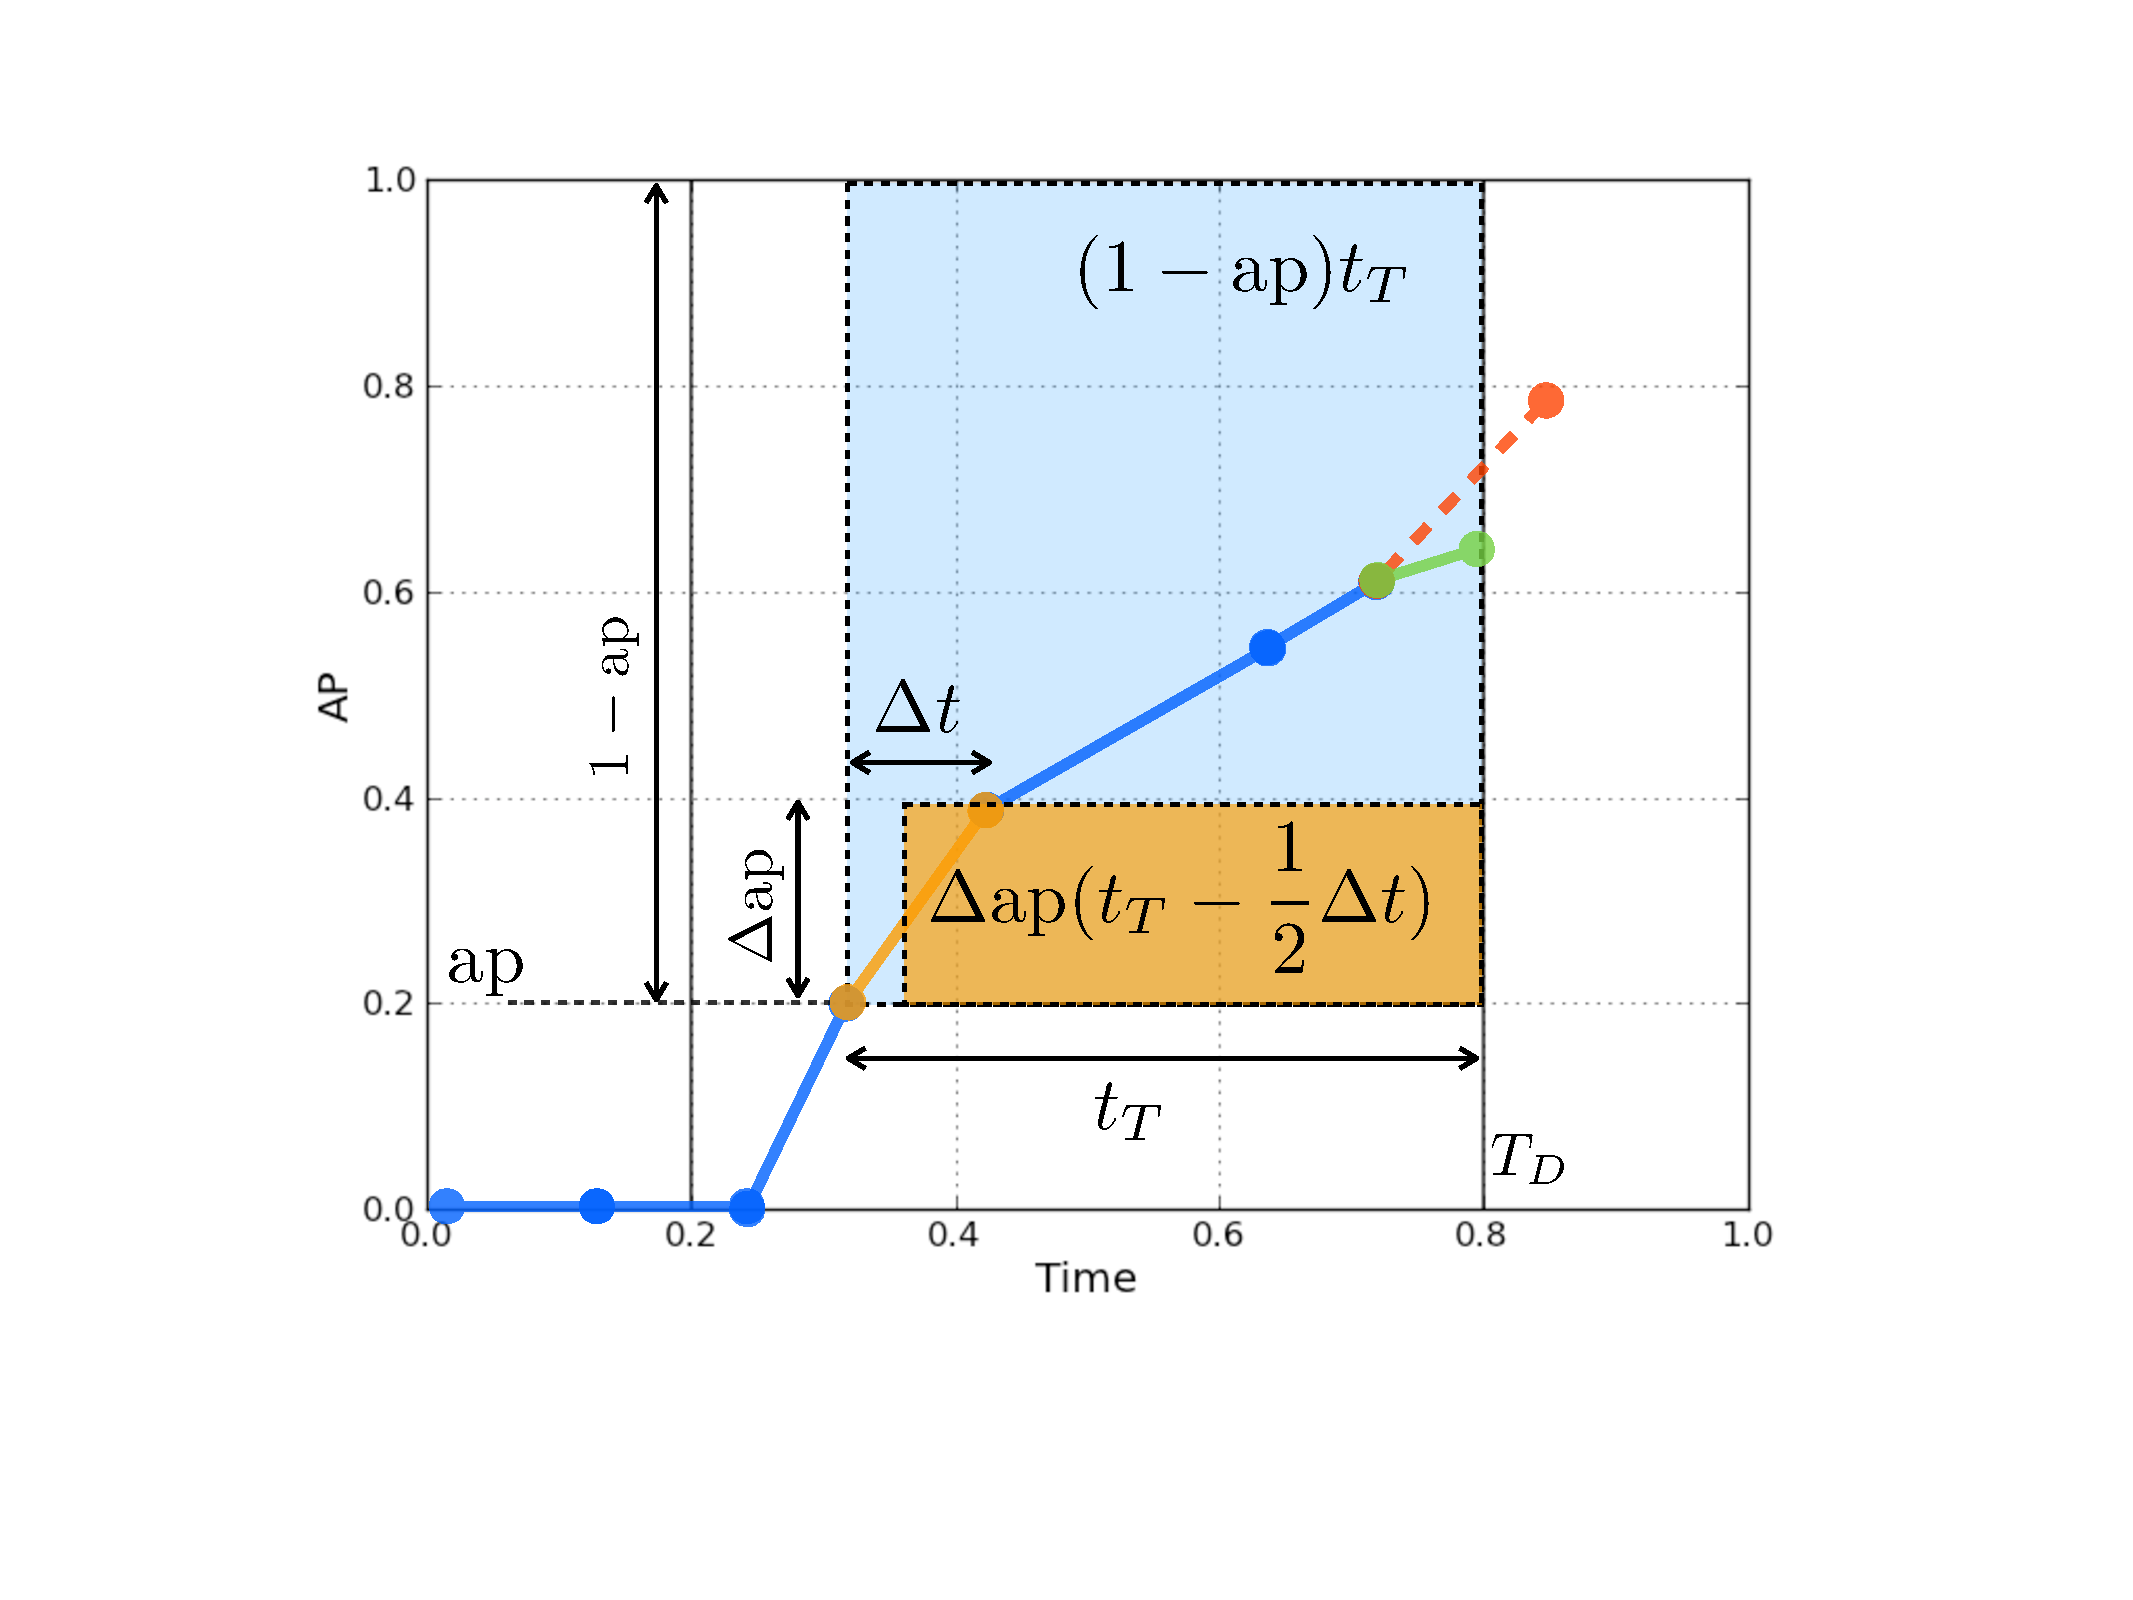
\includegraphics[height=10cm]{../../figures/apvst_expl.pdf}
      \end{center}}
      \\

      \begin{center}\textbf{Reinforcement Learning}\end{center}
      To compute $Q^\pi(s^j,a) = \mathbb{E} [R \mid s, a, \pi)]$, where $R = \sum_{i=j}^J \gamma^{i-j} R(s^i,a^i)$ and $J$ is the index of the last action before deadline time $T_d$, we run Monte Carlo policy iteration.
      We evaluate full episodes of the detection task on several thousand images, with a decreasing $\epsilon$-greedy policy.
      Policy weights $\theta$ are updated with $L_2$ regularization.

      \paragraph{}
      We evaluate different values of the reward discount $\gamma$, which at $0$ induces a completely greedy policy, and at $1$ has full lookahead.
      We find $\gamma = 0.4$ to work best in cross-validation.
      \\

      \begin{center}\textbf{Feature Representation}\end{center}
      The features $\phi(s, a)$ are composed of\\

      {\small
      \begin{tabularx}{0.8\linewidth}{p{0.23\linewidth}p{0.69\linewidth}}
      $P(C_a)$ & The prior probability of presence of the class that corresponds to the detector of action $a$ (omitted for the scene-context action).\\

      $P(C_0|\mathbf{o}) \ldots P(C_K|\mathbf{o})$ & The presence probabilities for all classes, conditioned on the current set of observations.\\

      $H(C_0|\mathbf{o}) \ldots H(C_K|\mathbf{o})$ & The entropies for all classes, conditioned on the current set of observations. \\

      $t^j_T$ & The time until deadline, and four other time features.\\
      \end{tabularx}
      }\\\\

      \begin{center}\textbf{Updating the belief state}\end{center}
      Observations $\mathbf{o}$ of detector for class $k$ update $P(C_k|\mathbf{o})$ either \emph{directly} (using a probability estimated by a classifier trained on the detector output) or through an \emph{MRF}.
      The MRF is learned with $L_1$-regularization and inference is done with loopy belief propagation.

    }; \addcenteredtitle{model}{Learning the Policy}

    % ==============================================================================
    % RESULTS
    \path (model.north east) ++(2cm,0cm) node(results) [style=tbox,text width=30cm] {
    We evaluated on the PASCAL VOC 2007 detection task, with 20 Deformable Part Model detectors (one per class), and an additional
    scene context action (GIST feature).
    \\

    We compared against a random baseline, an optimal static ordering, and an oracle ordering.

    \parbox{12cm}{
    \textbf{Weights} Learning with a higher $\gamma$ results in policies more relient on the global scene feature, for example.}%
    \parbox{18cm}{\hfill
    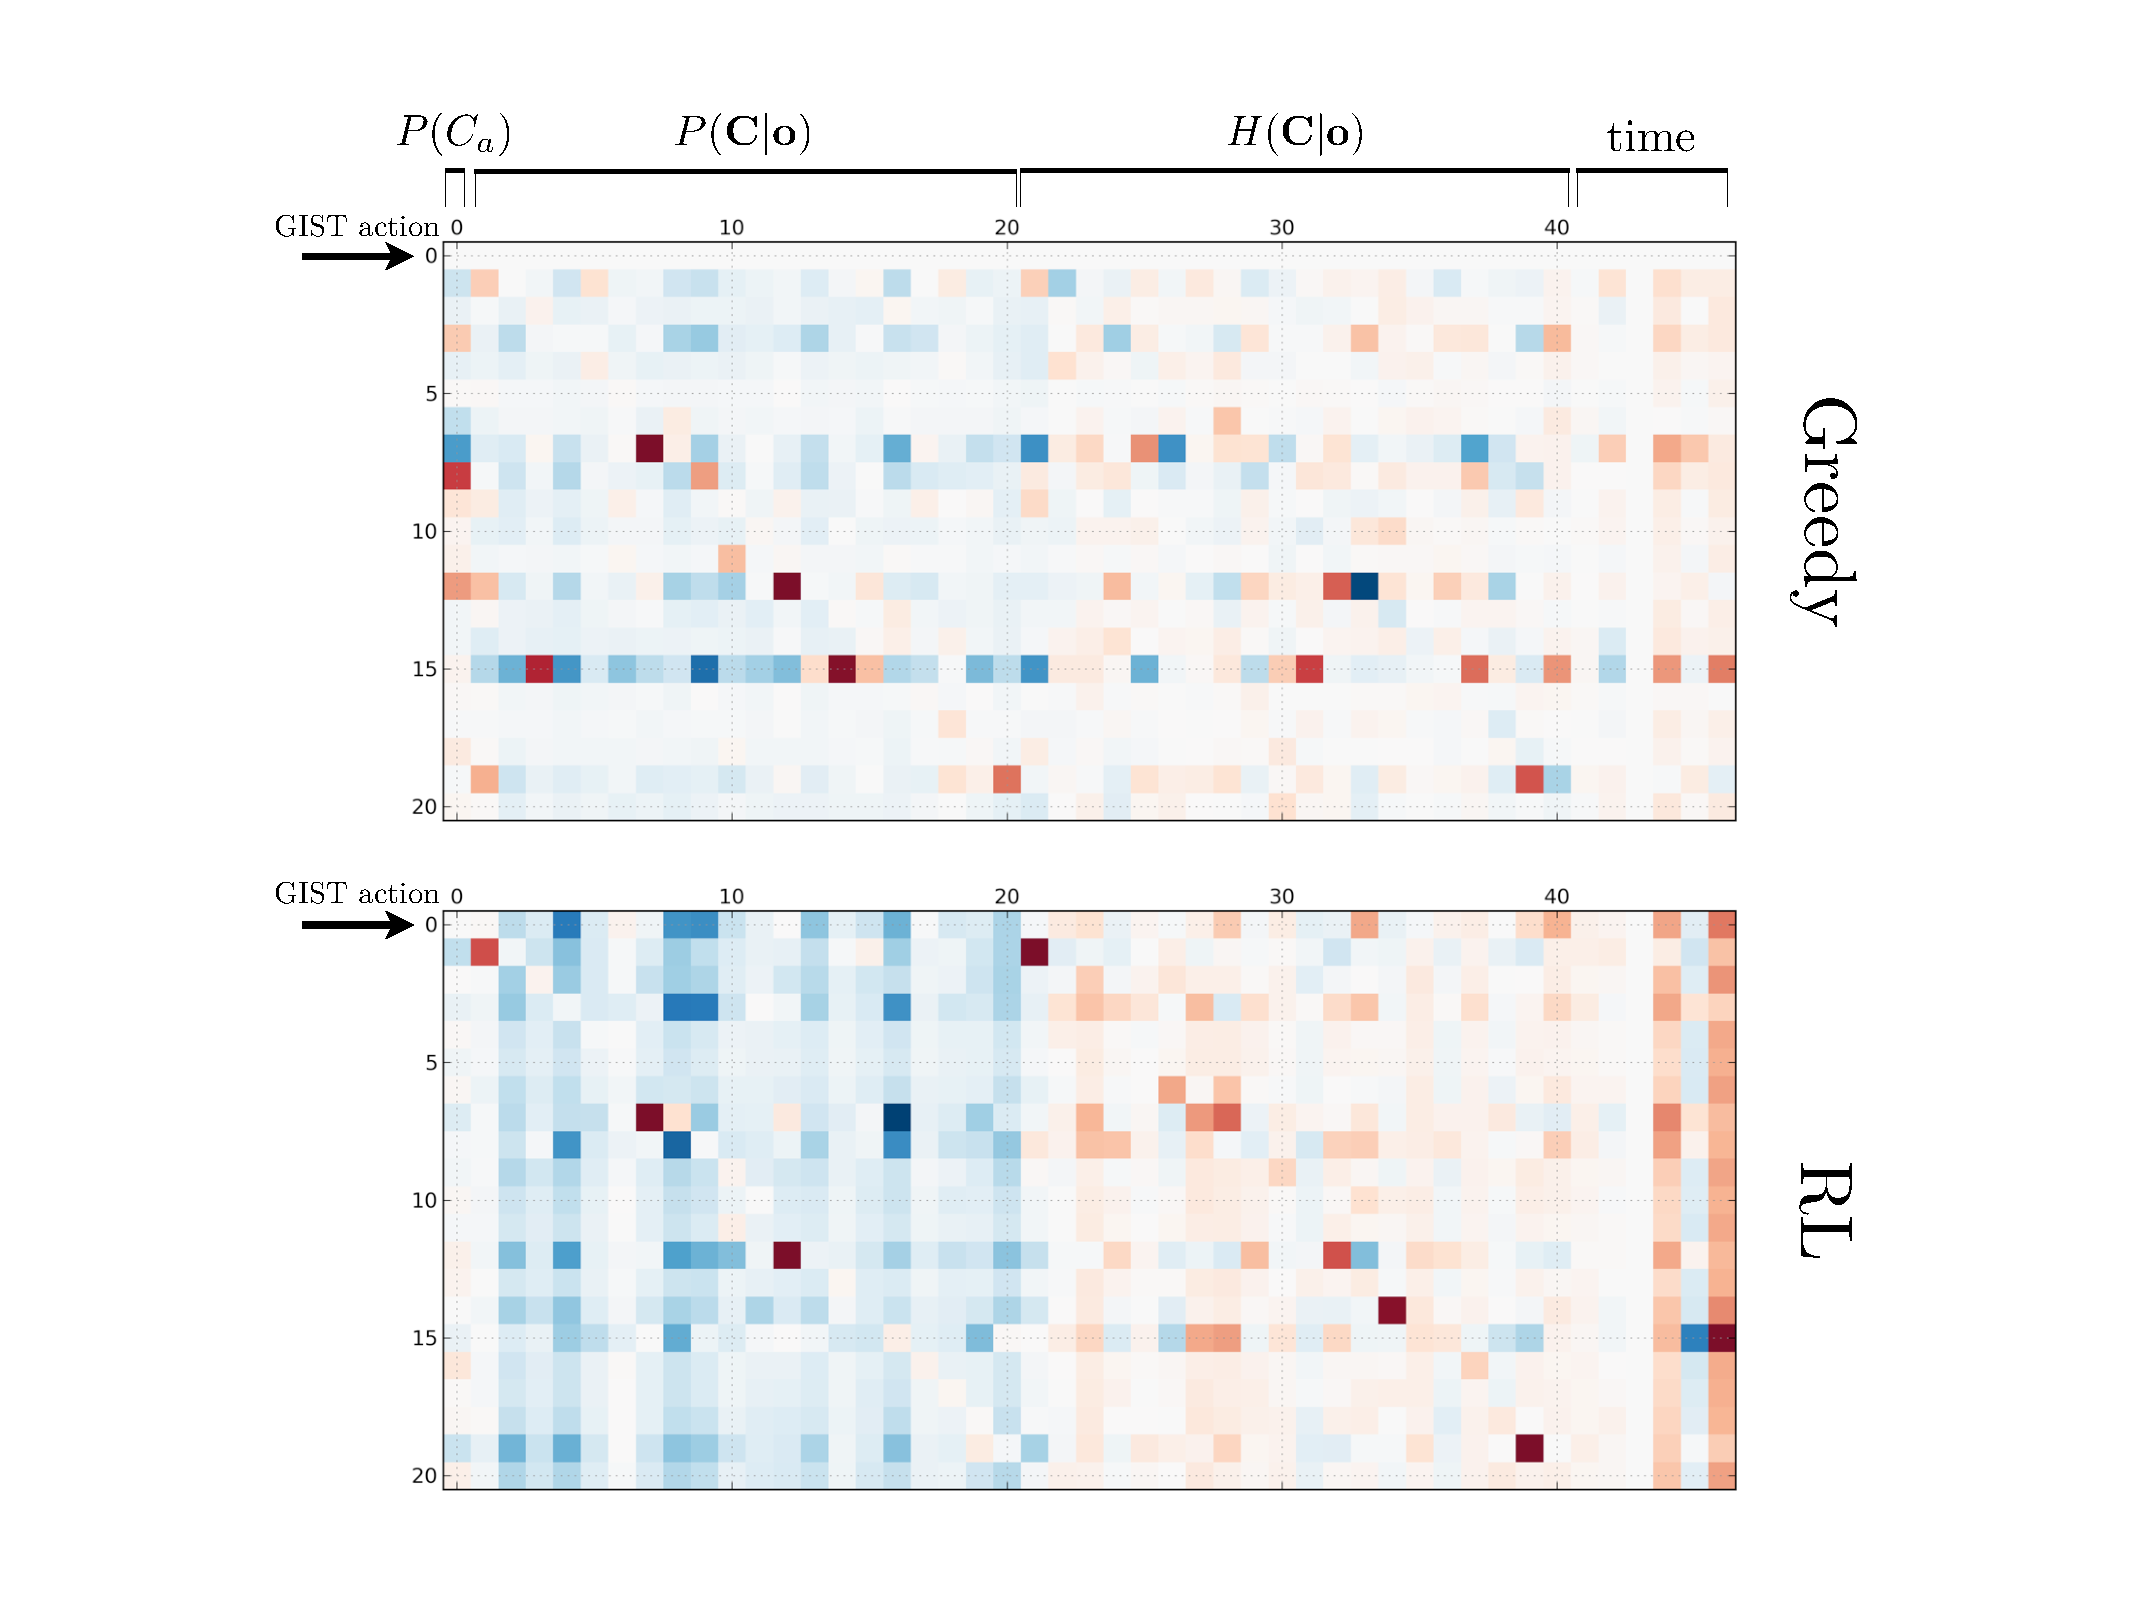
\includegraphics[width=17cm]{../../figures/weights.pdf}}
    \\

    \parbox{18cm}{
    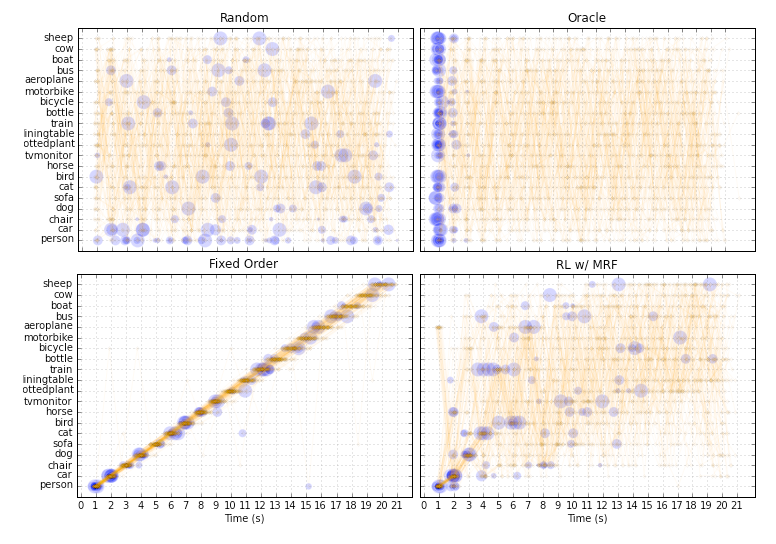
\includegraphics[width=17cm]{../../figures/trajectories.pdf}}%\hfill
    \parbox{12cm}{
    \textbf{Trajectories} Action selection traces are plotted in orange over many episodes; the size of the blue circles correspond to the increase in AP obtained by the action. Our policy does not stick a static order but selects actions dynamically to maximize the rewards obtained early on.}
    \\\\

    \parbox{18cm}{
    \textbf{Performance vs. Time}\\
    If execution is stopped when only half the detectors have been run, our method obtains 66\% better AP than a random ordering, and 14\% better performance than an intelligent baseline. On the timeliness measure, our method obtains at least 11\% better performance}
    \parbox{12cm}{\hfill
    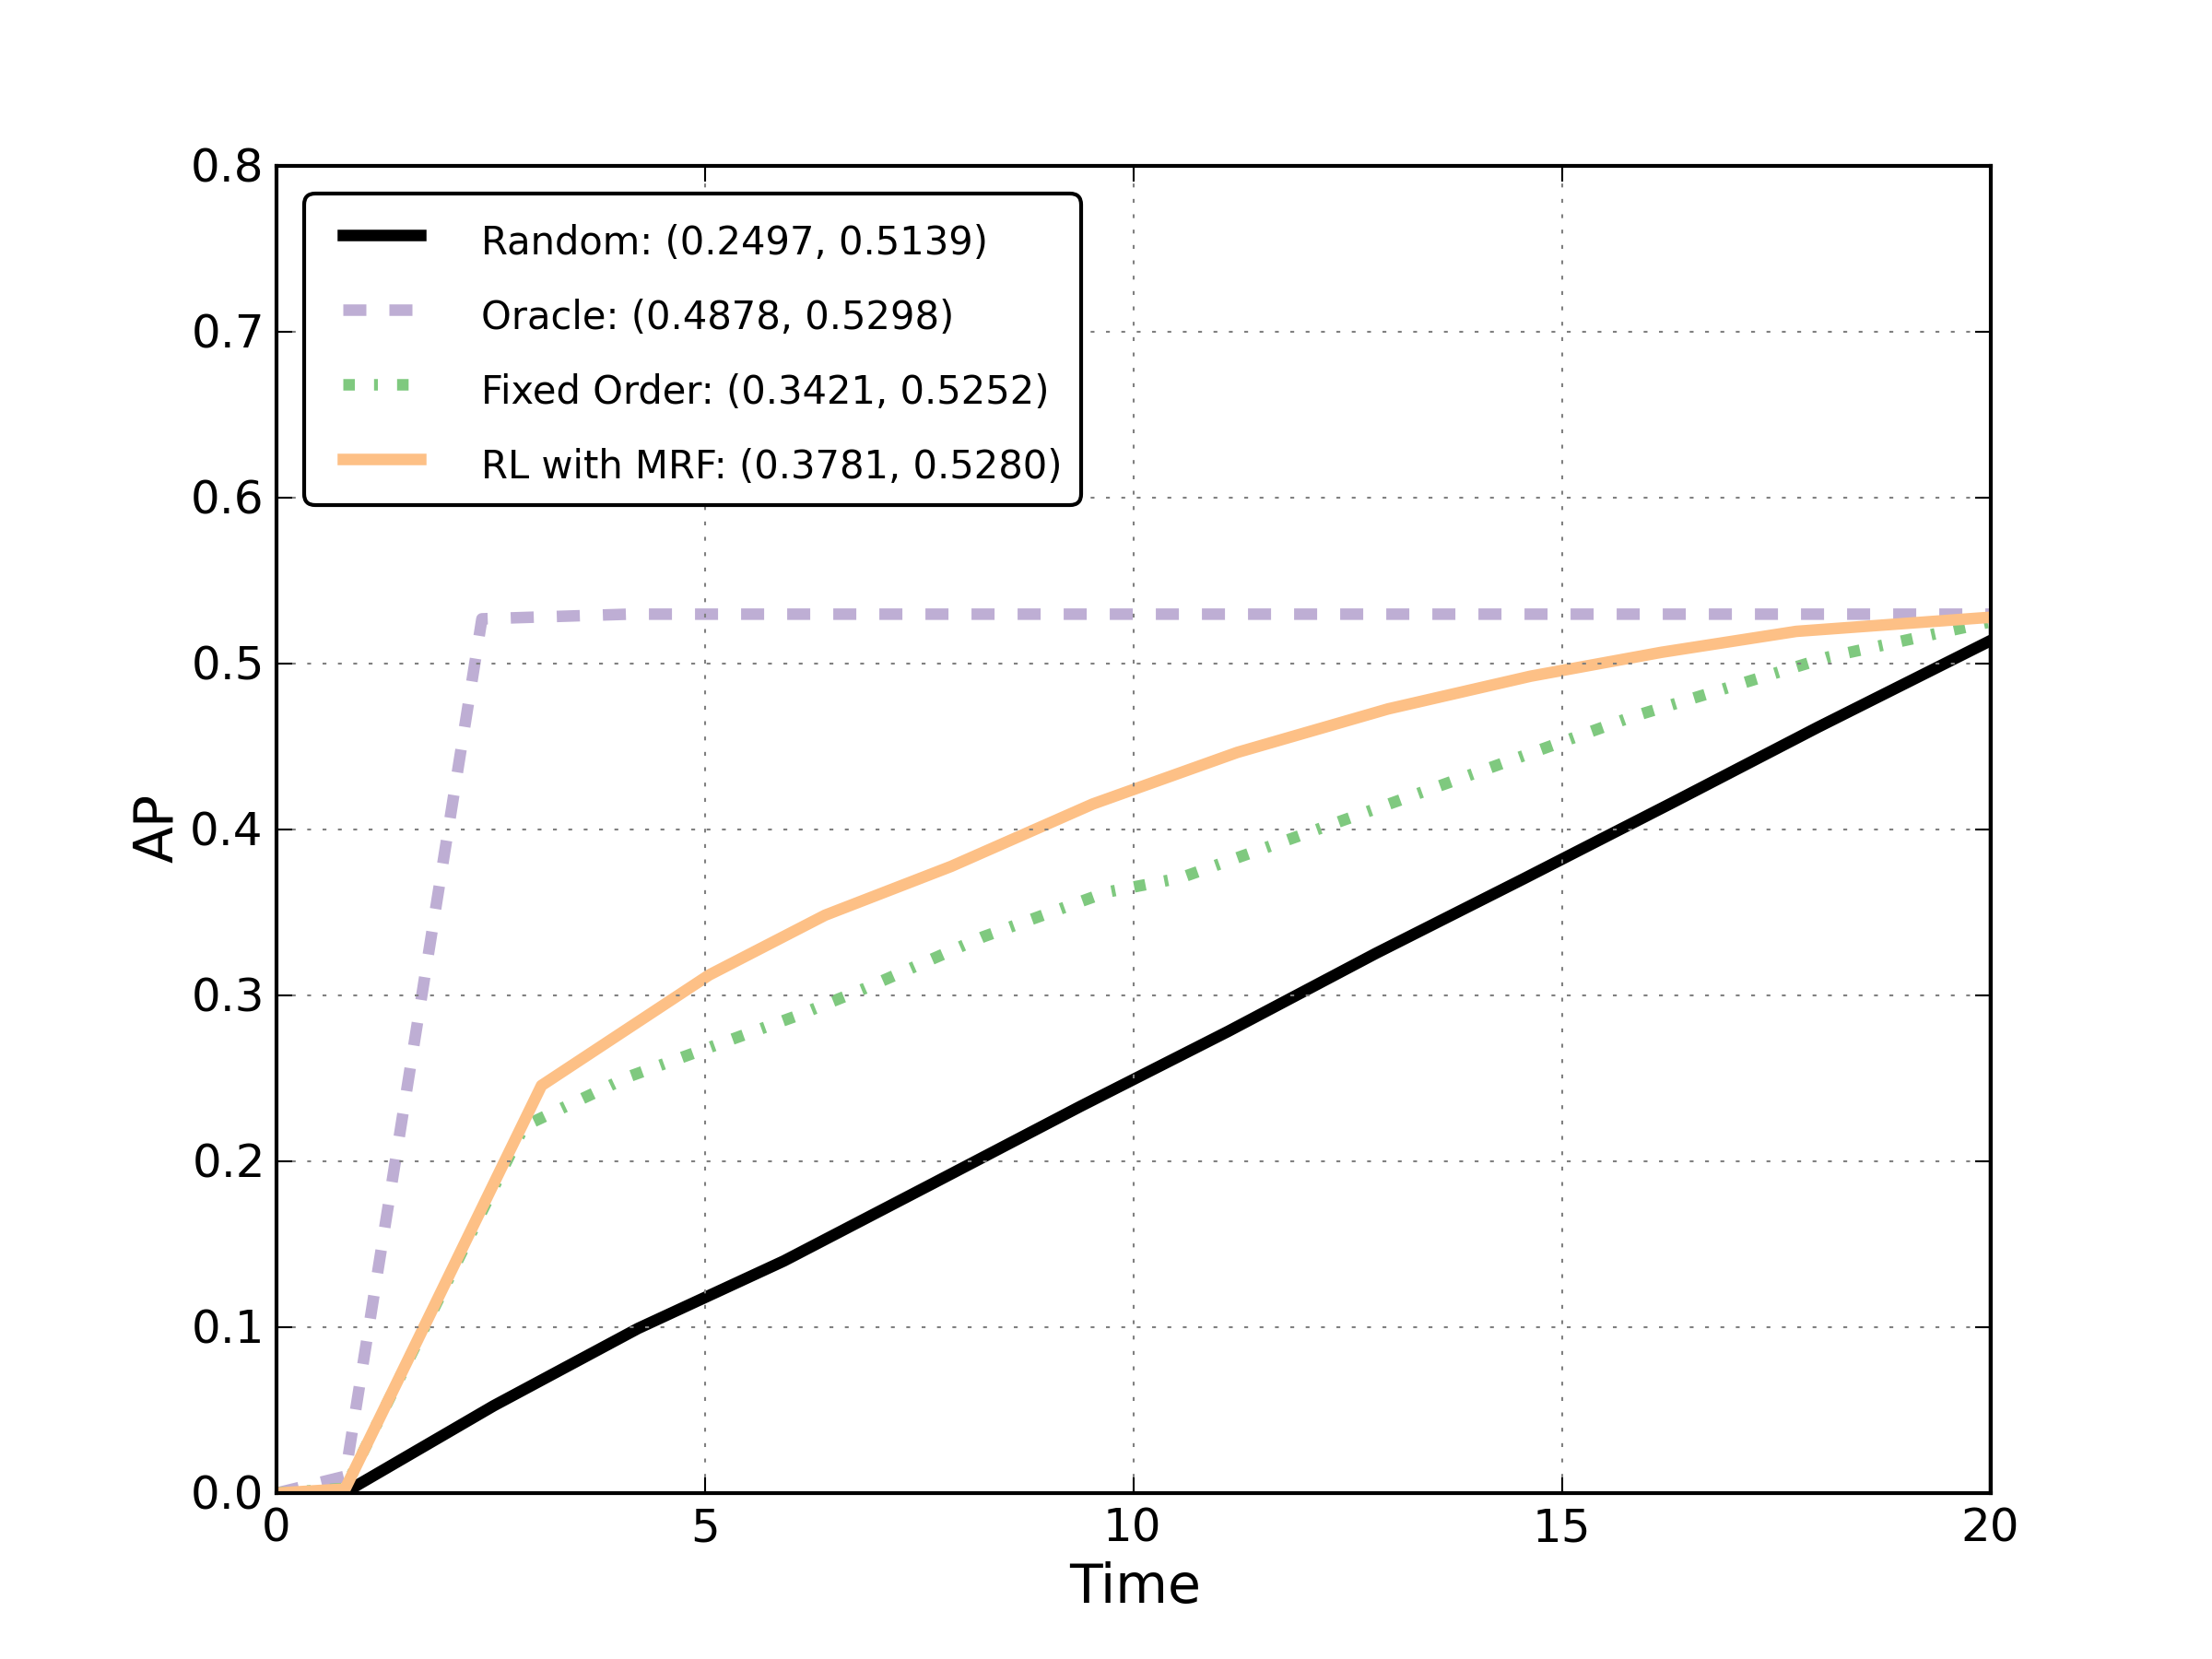
\includegraphics[width=11cm]{../../figures/final1.png}}%\hfill
    \\

    \begin{center}
    \begin{tabular}{|c|c|c|c|c|c|}
    \hline
    Bounds & Random & Fixed Order & RL        & RL w/ GIST         & Oracle \\ \hline
    (0,20) & 0.250  & 0.342       & 0.378     & \textbf{0.382}  & 0.488 \\ 
    (0,10) & 0.119  & 0.240       & 0.266     & \textbf{0.267}  & 0.464 \\ 
    (5,15) & 0.257  & 0.362       & 0.418     & \textbf{0.420}  & 0.530 \\ \hline
    \end{tabular}
    \end{center}

    }; \addcenteredtitle{results}{Results}
    
\end{tikzpicture}

\end{center}
\end{document}



